\documentclass[10pt,a4paper]{article}
\usepackage[utf8]{inputenc}
\usepackage[german]{babel}
\usepackage{amsmath}
\usepackage{amsfonts}
\usepackage{amssymb}
\usepackage{siunitx}
\usepackage[left=2cm,right=2cm,top=2cm,bottom=2cm]{geometry}
\usepackage{wrapfig}
\usepackage{graphicx}
\usepackage[outdir=./figures/]{epstopdf}
\usepackage{caption}
\usepackage[colorlinks]{hyperref}
\usepackage{pdflscape}

\author{Christian Bespin \and Christopher Deutsch}
\title{Übungsblatt 4: Numerische Methoden der Physik}
\begin{document}
\maketitle

\setcounter{section}{1}

\section{Widerstandswürfel}

\subsection{Physikalischer Hintergrund}

In vielen elektronischen Schaltungen finden sich ohm'sche Widerstände, deren Betrachtung hier im Vordergrund steht. Zum Verständnis der Schaltungen ist es interessant, das Verhalten der Widerstände zu kennen. Bei der Bearbeitung der Aufgaben werden Widerstandsnetzwerke berechnet. Dies lässt sich analytisch durchführen, in dem man Widerstände in Parallel- bzw. Reihenschaltungen zu Ersatzwiderständen zusammenfasst, bis man schlussendlich einen Ersatzwiderstand für die gesamte Schaltung erhält. Zur Berechnung nutzt man nun, dass sich Widerstände in Parallelschaltung reziprok und in Reihenschaltung gewöhnlich addieren (s. \ref{auswertung} für die hier benötigten analytischen Berechnungen).

Numerisch lässt sich ein Widerstandsnetzwerk aus einem linearen Gleichungssystem bestimmen. Zur Berechnung des Gesamtwiderstands werden die einzelnen Widerstände in Relationen zueinander gestellt. Es gilt allgemein das Faraday'sche Induktionsgesetz für stationäre Ströme
\begin{align}
\oint_{\partial\Sigma} \vec{E}\,\mathrm{d}\vec{l}=-\frac{\mathrm{d}}{\mathrm{dt}}\iint_{\Sigma}\vec{B}\,\mathrm{d}\vec{S}
\end{align}
wobei die rechte Seite gleich $0$ ist, da wir eine Gleichspannung anlegen und somit Ströme auftreten, die ein konstantes Magnetfeld $\vec{B}$ erzeugen. Daraus folgt mit der Tatsache, dass das Linienintegral über $\vec{E}$ einer Spannung entspricht, unmittelbar die Kirchhoff'sche Maschenregel $\sum_i U_i=0$, nach der sich alle Spannungen in einer Masche des Netzwerks aufheben.
Die Spannungen an den Widerständen werden mit dem Ohmschen Gesetz ($U=R I$) aus $I$ und $R$ berechnet. Es lassen sich im Fall des Würfels $6$, beim Oktaeder $8$ Maschen finden, für die je eine Gleichung aufgestellt wird, mit denen sich ein lineares Gleichungssystem in Matrixschreibweise aufstellen lässt (REFS). Wir berechnen also den Vektor mit Komponenten $I_i, I_{ges}$, um von dem Gesamtstrom mit erneuter Verwendung des Ohm'schen Gesetzes auf den Gesamtwiderstand $R_{ges}$ zu schließen.
Neben der Maschenregel existiert auch die Knotenregel, nach der die Summe der Ströme $I$ an einem Knoten des Netzwerks gleich $0$ ist (es sind die Richtungen der Ströme zu beachten). Sie folgt aus der Kontinuitätsgleichung $\frac{\partial\rho}{\partial t}+\mathrm{div}\vec{j}=0$.
Maschen- und Knotenregel bilden zusammen die Grundlage zur Analyse beliebiger Netzwerke.

\subsection{Lösung des linearen Gleichungssystems}
Wir haben ein lineares Gleichungssystem der Form $A\vec{x} = \vec{b}$. Jede invertierbare Matrix $A$ lässt sich durch $LR = PA$ darstellen. Dabei ist $L$ eine Untere und $R$ eine obere Dreiecksmatrix. Die Permutationsmatrix $P$ entsteht durch die Pivotisierung der Reihen.

Damit lässt sich das Gleichungssystem ausdrücken als $PA\vec{x} = LR\vec{x} = P\vec{b}$. Jetzt kann schrittweise die Lösung des Gleichungssystems berechnet werden, indem man das Gleichungssystem als $L\vec{y} = P\vec{b}$ mit $\vec{y} = R\vec{x}$ schreibt. Zunächst berechnet man $\vec{y}$ durch Vorwärtssubstitution, um dann aus $R\vec{x} = \vec{y}$ die Lösung des Gleichungssystems durch Rückwärtssubstitution zu erhalten.

\subsubsection{LR-Zerlegung}
Wir zerlegen eine Matrix $A$ in ein Produkt aus unterer und oberer Dreiecksmatrix, indem wir die Matrix $A$ mithilfe des Gauß'schen Eliminationsverfahrens auf obere Dreiecksform bringen. Die Umformungsschritte des Eliminationsverfahrens können durch die Elementarmatrix $Q^j_i(\lambda)$ beschrieben werden. Dabei beschreibt $Q^j_i (\lambda) A$ die Addition des $\lambda$-fachen der $j$-ten Zeile von $A$ zur $i$-ten Zeile. Konkret hat $Q^j_i (\lambda)$ die Form der Einheitsmatrix mit Ausnahme von $\left(Q^j_i (\lambda) \right)_{i, j} = \lambda$. Das Inverse dieser Matrix ist gegeben durch $\left( Q^j_i\right) ^{-1} (\lambda) = Q^j_i (-\lambda)$.

Wir können jetzt eine LR-Zerlegung einer ($N \times N$)-Matrix $A$ durchführen, indem wir zunächst das Gauß'sche Eliminationsverfahren auf die erste Spalte der Matrix $A = A^{(0)}$ anwenden und diese damit in die Matrix $A^{(1)}$ überführen. Mit der oben beschriebenen Elementarmatrix und ihrer Inversen können wir offenbar schreiben:
\begin{align}
	A^{(0)} = \prod_{k=2}^N Q^1_k \left( \frac{(A)_{k,1}}{(A)_{1,1}}\right)  A^{(1)}
\end{align}
Insbesondere sind die Elementarmatrizen alle von unterer Dreickecksform und damit das Produkt von unteren Dreiecksmatrizen auch wieder eine untere Dreiecksmatrix. Dieses Verfahren wird solange für die nachfolgenden Spalten durchgeführt, bis $A^{(N-1)} = R$ obere Dreiecksform hat. Somit haben wir die Matrix $A = L R$ als ein Produkt von unterer und oberer Dreiecksmatrix ausgedrückt. 

Die Zerlegung wurde in der Funktion \texttt{LU\_decomp} implementiert. Insbesondere hat die Matrix $L$ als Produkt von Elementarmatrizen nur Einsen auf ihrer Hauptdiagonalen, weshalb wir diese nicht explizit speichern müssen. Dies legt nahe, dass wir die Matrix $L$ in den durch das Gauß'sche Eliminationsverfahren eliminierten Matrixelementen speichern.


\subsubsection{Oktaeder}

\subsection{Implementierung}

\subsubsection{Nullstellenberechnung mit Bisektion}

\subsubsection{Numerische Integration mit rekursivem Simpson-Verfahren}


\subsubsection{Abbruchbedingungen}

\subsubsection{Genaugkeit}

\subsection{Physikalische Ergebnisse}

\subsubsection{Analytische Lösung für gleiche Widerstände}
\label{auswertung}
\begin{wrapfigure}[19]{R}[1pt]{0.32\textwidth}
\centering
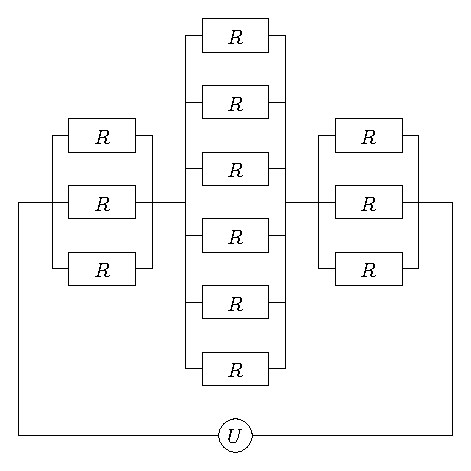
\includegraphics[width=0.3\textwidth]{./figures/ersatzschaltbild.eps}
\caption{Schaltbild für gleiche Widerstände $R$}
\label{fig:ersatzschaltbild}
\end{wrapfigure}
Für den Fall, dass alle verwendeten Widerstände gleich sind, lassen sich alle Ecken gleichen Potenzials verbinden und man erhält ein einfaches Ersatzschaltbild (Abb. \ref{fig:ersatzschaltbild}). Man nutzt nun aus, dass sich Widerstände in Parallelschaltungen reziprok und in Reihenschaltungen gewöhnlich addieren. Man erhält somit schnell:
\begin{align}
R_{ges}=\frac{R}{3}+\frac{R}{6}+\frac{R}{3}=\frac{5}{6}\,R
\end{align}

Für die Aufgabe gleicher Widerstände erhalten wir numerisch die gleiche Lösung, die sich bei analytischer Betrachtung ergibt. Zusammengefasst erhalten wir:
\begin{table}[htbp!]
\centering
\begin{tabular}{l|l}
Geometrie und Schaltung & Gesamtwiderstand $R_{ges}$\\\hline
\\
Würfel, Raumdiagonale & $5/6$
\end{tabular}
\end{table}


\begin{thebibliography}{9}

\bibitem{lyness}
 Lyness, J. N.,
 \emph{Notes on the Adaptive Simpson Quadrature Routine},
Journal of the ACM
Volume 16 Issue 3, (1969) 
Seiten 483-495 

\end{thebibliography}
\begin{landscape}
\thispagestyle{empty}
\appendix
\section{Anhang}
\subsection{Würfel}
\begin{figure}[htbp!]
\centering
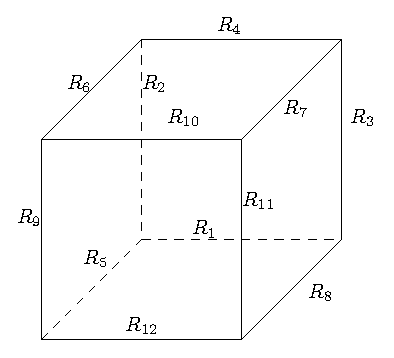
\includegraphics{./figures/wuerfel.eps}
\caption{Geometrie des Würfels mit Festlegung der Widerstände}
\label{fig:geometrie_wuerfel}
\end{figure}
\subsubsection{Spannung an der Raumdiagonalen}
\begin{align}
\begin{pmatrix}
R_1+R_2+R_3+R_4 &  -R_4  &  0  &  -R_3  &  -R_2  &  0  \\ 
-R_4 & R_4+R_6+R_7+R_{10} & -R_{10} & -R_7 & -R_6 & -R_6 \\ 
 0  & -R_{10} & R_9+R_{10}+R_{11}+R_{12} & -R_{11} & -R_9 & -(R_9+R_{12}) \\ 
-R_3 & -R_7 & -R_11 & R_3+R_7+R_8+R_{11} & 0 & 0 \\ 
-R_2 & -R_6 & -R_9 & 0 & R_2+R_5+R_6+R_9 & R_6+R_9 \\ 
 0  & -R_6 & -(R_9+R_{12}) &  0  & R_6+R_9 & R_6+R_9+R_{12}
\end{pmatrix}
\begin{pmatrix}
I_1\\I_2\\I_3\\I_4\\I_5\\I_{ges}
\end{pmatrix}
=
\begin{pmatrix}
0\\0\\0\\0\\0\\U
\end{pmatrix}
\label{eqn:wuerfel_ganz}
\end{align}

\begin{figure}[htbp!]
\centering
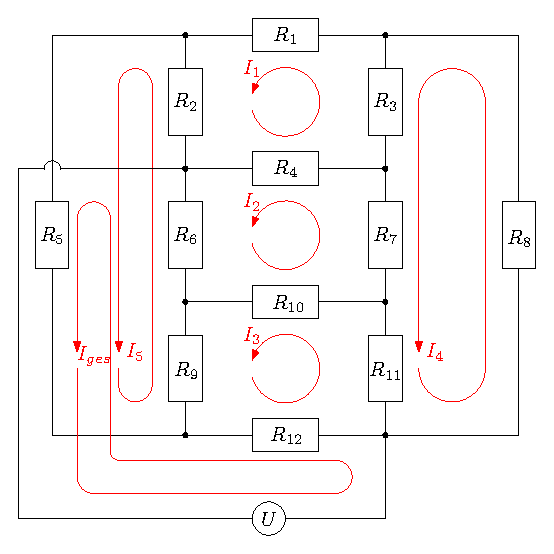
\includegraphics{./figures/wuerfel_schaltplan.eps}
\caption{Schaltplan eines Widerstandswürfels mit angelegter Spannung an einer Raumdiagonalen}
\label{fig:wuerfel_schaltplan}
\end{figure}

\subsubsection{Spannung an der Flächendiagonalen}
\thispagestyle{empty}
\begin{align}
\begin{pmatrix}
R_1+R_2+R_3+R_4 &  -R_4  &  0  &  -R_3  &  -R_2  &  0  \\ 
-R_4 & R_4+R_6+R_7+R_{10} & -R_{10} & -R_7 & -R_6 & -R_6 \\ 
 0  & -R_{10} & R_9+R_{10}+R_{11}+R_{12} & -R_{11} & -R_9 & -R_9 \\ 
-R_3 & -R_7 & -R_11 & R_3+R_7+R_8+R_{11} & 0 & 0 \\ 
-R_2 & -R_6 & -R_9 & 0 & R_2+R_5+R_6+R_9 & R_6+R_9 \\ 
 0  & -R_6 & -R_9 &  0  & R_6+R_9 & R_6+R_9
\end{pmatrix}
\begin{pmatrix}
I_1\\I_2\\I_3\\I_4\\I_5\\I_{ges}
\end{pmatrix}
=
\begin{pmatrix}
0\\0\\0\\0\\0\\U
\end{pmatrix}
\label{eqn:wuerfel_flaeche}
\end{align}

\begin{figure}[htbp!]
\centering
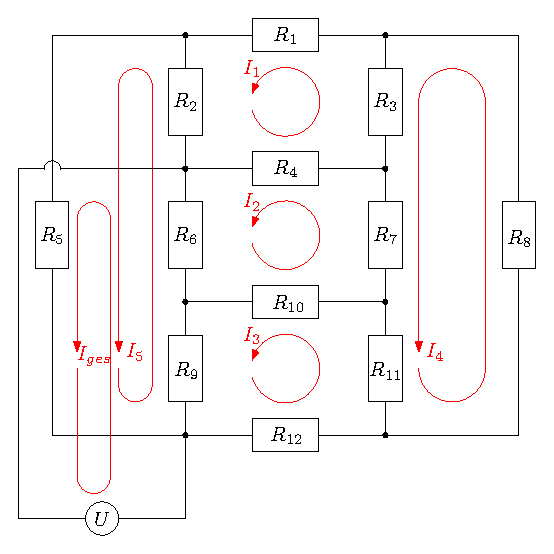
\includegraphics{./figures/wuerfel_schaltplan_flaeche.eps}
\caption{Schaltplan eines Widerstandswürfels mit angelegter Spannung an einer Flächendiagonalen}
\label{fig:wuerfel_schaltplan_flaeche}
\end{figure}

\subsubsection{Spannung an einer Kante}
\begin{align}
\begin{pmatrix}
R_1+R_2+R_3+R_4 &  -R_4  &  0  &  -R_3  &  -R_2  &  0  \\ 
-R_4 & R_4+R_6+R_7+R_{10} & -R_{10} & -R_7 & -R_6 & 0 \\ 
 0  & -R_{10} & R_9+R_{10}+R_{11}+R_{12} & -R_{11} & -R_9 & -R_{12} \\ 
-R_3 & -R_7 & -R_11 & R_3+R_7+R_8+R_{11} & 0 & 0 \\ 
-R_2 & -R_6 & -R_9 & 0 & R_2+R_5+R_6+R_9 & 0 \\ 
 0  & 0 & -R_{12} &  0  & 0 & R_{12}
\end{pmatrix}
\begin{pmatrix}
I_1\\I_2\\I_3\\I_4\\I_5\\I_{ges}
\end{pmatrix}
=
\begin{pmatrix}
0\\0\\0\\0\\0\\U
\end{pmatrix}
\label{eqn:querfel_kante}
\end{align}
\thispagestyle{empty}
\begin{figure}[htbp!]
\centering
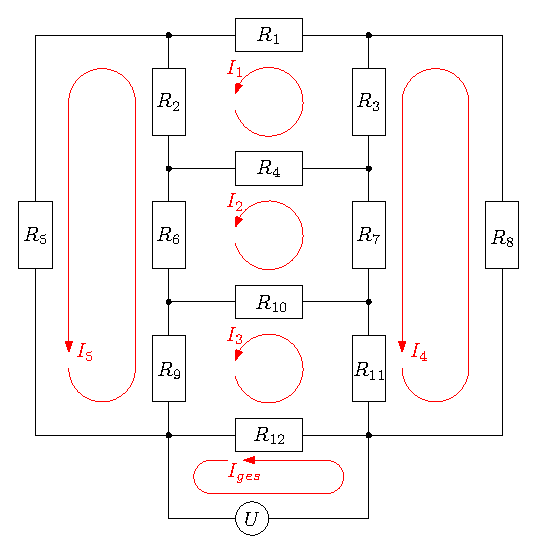
\includegraphics{./figures/wuerfel_schaltplan_kante.eps}
\caption{Schaltplan eines Widerstandswürfels mit angelegter Spannung an einer Kante}
\label{fig:wuerfel_schaltplan_kante}
\end{figure}
\subsection{Oktaeder}
\begin{figure}[htbp!]
\centering
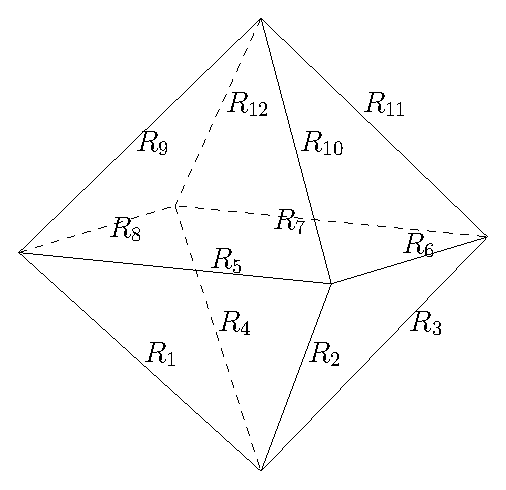
\includegraphics{./figures/oktaeder.eps}
\caption{Geometrie des Oktaeders mit Festlegung der Widerstände}
\label{fig:geometrie_oktaeder}
\end{figure}
\subsubsection{Spannung an der Diagonalen}
\begin{align}
\begin{pmatrix}
	0 & 0 & -R_4 & 0 & 0 & -R_{12} & 0 & R_4 + R_{12} \\
	R_1 + R_2 + R_5 & -R_2 & 0 & -R_5 & 0 & 0 &-R_5 & 0 \\
	-R_2 & R_2 + R_3 + R_6 & -R_3 & 0 & -R_6 & 0 & -R_6 & 0 \\
	0 & -R_3 & R_3 + R_4 + R_7 & 0 & 0 & -R_7 & -R_7 & -R_4 \\
	-R_5 & 0 & 0 & R_5 + R_9 + R_{10} & -R_{10} & 0 & R_5 & 0 \\
	0 & -R_6 & 0 & -R_{10} & R_6 + R_{10} + R_{11} & -R_{11} & R_6 & 0 \\
	0 & 0 & -R_7 & 0 & -R_{11} & R_7 + R_{11} + R_{12} & R_7 & -R_{12} \\
	-R_5 & -R_6 & -R7 & R_5 & R_6 & R_7 & R_5 + R_6 + R_7 + R_8 & 0
\end{pmatrix}
\begin{pmatrix}
I_1\\ I_2\\ I_3\\I_4\\I_5\\I_6\\I_7\\I_{ges}
\end{pmatrix}
=
\begin{pmatrix}
U\\0\\0\\0\\0\\0\\0\\0
\end{pmatrix}
\label{eqn:oktaeder_ganz}
\end{align}
\begin{figure}[htbp!]
\centering
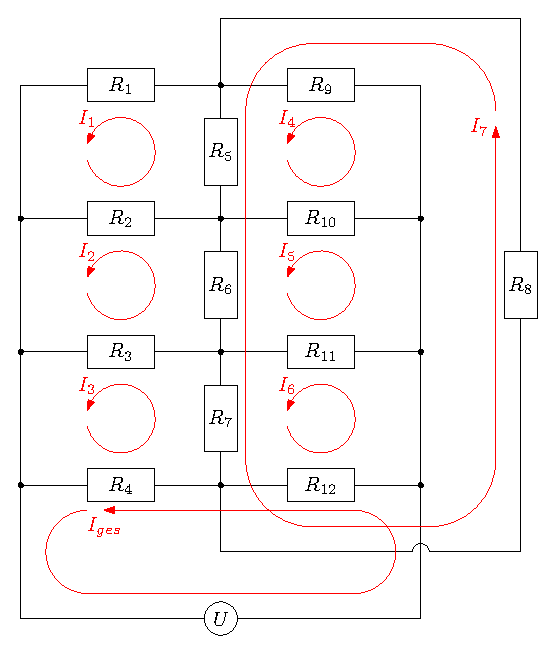
\includegraphics{./figures/oktaeder_schaltplan.eps}
\caption{Schaltplan eines Oktaeders mit angelegter Spannung an der Diagonalen}
\label{fig:oktaeder_schaltplan}
\end{figure}
\thispagestyle{empty}
\subsubsection{Spannung an einer Kante}
\begin{figure}[htbp!]
\centering
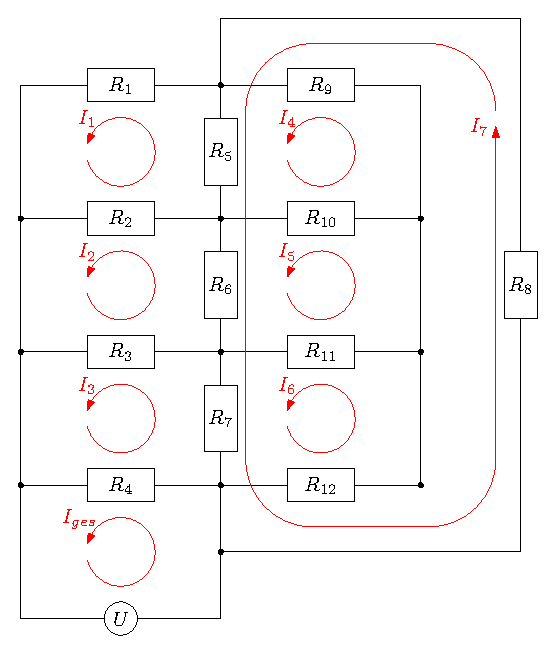
\includegraphics{./figures/oktaeder_schaltplan_kante.eps}
\caption{Schaltplan eines Oktaeders mit angelegter Spannung an einer Kante}
\label{fig:oktaeder_schaltplan_kante}
\end{figure}
\end{landscape}



\end{document}
